\chapter{Client-Server Architecture}

\section{Basic notions}

This section presents some basic notions useful to understand this chapter.

\subsection{Application, libraries and build}

An application is a set of routines that one can execute to do a specific task.
An application is an executable file. \\

A library can be seen as an application that is not executable by itself. A
library contains routines that can be shared between multiple applications. In
other words, a library allows code centralization between several applications.
There are two main types of libraries :
\begin{itemize}
 \item static librairies : routines used by an application are copied into this
application executable during the linking (see below). If one the these routines
changes, the application need to be recompiled to get this change.
 \item dynamic libraries : unlike static librairies, the routines are not
copied during the linking (see below) but are called by the application during
runtime. Modifying a routine in a dynamic library will change the behaviour of
the applications that use it, maybe without modify them.
\end{itemize}

Both application and library are built from source code. The building process is
composed of two steps : 
\begin{itemize}
 \item the compilation : translation from a source file (the code) to an object
file. One object file is produced for each source file. This is done by a
\textit{compiler}.
 \item the linking : this step puts object files together to make a single file
which is either an application or a library. During this step, routines defined
in a library are copied (for a static library) into the file or, in the case of
a dynamic library, a \textit{link} is created between the file and the library.
This step is done by the \textit{linker}.
\end{itemize}

\subsection{\textit{Client} and \textit{server} notions}

A server is a program that can recieve requests and reply to them. A client is
a program that sends requests to a server and gets the answers. A server
that supports multiple clients accepts more than one client at a time.
Both server and client communicate through the network and don't have to be 
necessarily running on the same computer.\\

An example of a client application is a Web browser. It sends requests to
servers over the Internet and recieves Web pages. The use of the term
\textit{server} does not mean that it only runs on a server computer simply that
it provides services. It can run on the same
computer as the client.

%----------------------------------------------------------------------------
%----------------------------------------------------------------------------

\subsection{Sockets}

To be able to communicate through the network, two applications need to open a
communication channel. This channel is called a \textit{socket}. There are
\textit{client sockets} and \textit{server sockets}. The difference between
these two types is that a \textit{client socket} can attempt to connect to a
\textit{server socket} but will nerver accept connections from other sockets.\\

A \textit{server socket} accepts connection requests from a \textit{client
socket} but will never attempt to connect to another socket. Once the connection
has been established, both applications can use the socket to read and write
data. Of course, an application can open several sockets at the same time and
can play both roles of client and server at the same time.\\

%----------------------------------------------------------------------------
%----------------------------------------------------------------------------

\subsection{Ports}

Since there are many applications using network on a computer, the socket can
not cover all network interface. Each application using network would indeed
read all data arriving on the network. This is heavy and unsecure. To avoid
this, each socket uses a \textit{port}, which can be seen as an open door on 
the computer.\\

If an application tries to connect to a port that is not open, the connection is
refused. So, the server has to be launched and have opened the appropriate port
to authorize a client connection. On its side, the client opens its socket
on same port as the server. \\

A server application can not open a port that is already open. Multiple client
applications can open the same port on the same machine.\\

Each port is identified by a number from 0 to 65535. There are some rules
in the port assignement : 

\begin{itemize}
 \item Port numbers from 0 to 1023 are reserved and forbidden to use. 
 \item Port numbers from 1024 to 49152 are available but some are reserved, so
it is not recommended to use them (to avoid conflicts).
 \item Port numbers from 49153 to 65535 are free to use.\\
\end{itemize}

%----------------------------------------------------------------------------
%----------------------------------------------------------------------------

\subsection{Protocol}

A protocol is a set of rules established between two communicating entities and
that is understood by these entities. When two applications communicate through
a socket, the protocol concerns two things :

\begin{itemize}
 \item Requests order. A request may need to be executed before another. For
example : a client can not request a server to read a file if it has not been
open before.
 \item Data format. For example : a server supposed to recieve Microsoft
Word files can not recieve a simple text file, because data are not written in
the same way in the file.\\
\end{itemize}

The protocol used in my project is written in XML (\textit{e\textbf{X}tensible
\textbf{M}arkup \textbf{L}anguage}). XML is a language used to store and
transfer tree-structured data. The protocol is detailled in
\inQuotes{\textit{Annexes - Volume 3 : Network Protocol}}.

%++++++++++++++++++++++++++++++++++++++++++++++++++++++++++++++++++++++++++++
%++++++++++++++++++++++++++++++++++++++++++++++++++++++++++++++++++++++++++++
%++++++++++++++++++++++++++++++++++++++++++++++++++++++++++++++++++++++++++++
%++++++++++++++++++++++++++++++++++++++++++++++++++++++++++++++++++++++++++++

\section{Project overview}

My project was to develop two applications and two dynamic librairies to provide
a graphical configuration tool for the simulations solved by \cf. These
applications and libraries are all written in C++ using Qt library.\\

The applications : 
\begin{itemize}
 \item client : the graphical user interface (GUI). Allows the user to
configure a simulation.
 \item server : forwards requests coming form the clients to the simulator. It
can be seen as an interface between the network and the simulator.\\
\end{itemize}

The libraries : 
\begin{itemize}
 \item network : centralizes the network protocol. Both client and server use 
it to build and parse network frames.
 \item treeview : provides tree management (in XML) for the client. This has
been detached from the client for portability convinience.\\
\end{itemize}

The project had two main phases :
\begin{enumerate}
 \item Develop a client-server simple XML communication.
 \begin{enumerate}
 \item The client sends a sentence entered by the user to the server.
 \item The server tranforms it to capital letters and sends the new string to
the client.
 \item The client recieves the string and displays it.
 \end{enumerate}
 The purpose of this phase was to establish a simple network communication using
XML frames format that would be used as a base for the next phase and take the
working environment in hand. The applications were not graphical.

 \item Develop the graphical user interface. This phase was evolutionary, adding
features one by one to the first phase. 
\end{enumerate}

%----------------------------------------------------------------------------
%----------------------------------------------------------------------------

\subsection{Network communication}

The clients have a copy of the configuration tree, handled by the simulator on
server side. Thus, each time the tree is modified by a client, all clients
connected to the same server application recieve the updated tree. There are
two kinds of communications with XML :
\begin{itemize}
 \item DOM XML : this is the communication between the server and the client.
The server sends always all the tree. When a client recieves it, it deletes the
old one and sets the new tree.
 \item SAX XML : this is the comunication between the client and the server.
The server never sends all the tree, but only the path of the part to modify
and the description of the modification to do (add or delete an object, add or
delete options,...).
\end{itemize}

%----------------------------------------------------------------------------
%----------------------------------------------------------------------------

\subsection{\cf notions}

\subsubsection{Tree, objects and options}

The simulation configuration is managed with an XML tree. Each node of this
tree is an object. This object has parameters to configure it, called
\textit{options}.

%----------------------------------------------------------------------------

\paragraph{Basic and advanced modes\\}

Object and options are either basic or advanced. Some users are not experienced
and do not need to see or use advanced options.

%----------------------------------------------------------------------------

\paragraph{Static and dynamic options\\}

An option is dynamic if the user can modify it during the simulation. Otherwise
it is static. Dynamic options are useful to refine or extend simulation
results, while the computation is running.

%----------------------------------------------------------------------------

\subsubsection{Configuration files}

A simulation configuration is written in a file. There are two possible
formats, depending on the file extension:
\begin{itemize}
 \item CFcase (\textit{\cf} case) : describes the simulation step by
step (modules to load, options and their values, ...).
 \item XCFcase (XML \textit{\cf} case) : equivalent to a CFcase file, but
written in XML.
\end{itemize}

Below, you can find a comparison between a portion in CFcase file and
the same portion in an XCFcase: \\

\begin{table}[H]
 \begin{lstlisting}
Simulator.SubSystem.OutputFormat = Tecplot CFmesh
Simulator.SubSystem.CFmesh.FileName = jets2DCRD.CFmesh
Simulator.SubSystem.Tecplot.FileName = jets2DCRD.plt
Simulator.SubSystem.Tecplot.Data.updateVar = Cons
Simulator.SubSystem.Tecplot.SaveRate = 1000
Simulator.SubSystem.CFmesh.SaveRate = 1000
Simulator.SubSystem.Tecplot.AppendTime = false
Simulator.SubSystem.CFmesh.AppendTime = false
Simulator.SubSystem.Tecplot.AppendIter = false
Simulator.SubSystem.CFmesh.AppendIter = false
 \end{lstlisting}
 \caption{Portion of a CFcase file}
\end{table}

\begin{table}[H]
\begin{lstlisting}
<XCFcase>
 <Simulator>
  (...)
  <SubSystem (...) OutputFormat="Tecplot CFmesh" (...)>
   <CFmesh AppendIter="false" AppendTime="false" FileName="jets2DCRD.CFmesh"
           SaveRate="1000"/>
   (...)
   <Tecplot AppendIter="false" AppendTime="false" FileName="jets2DCRD.plt"
            SaveRate="1000">
    <Data updateVar="Cons"/>
   </Tecplot>
  </SubSystem>
 </Simulator>
</XCFcase>
\end{lstlisting}
 \caption{Portion of an XCFcase file}
\end{table}


%----------------------------------------------------------------------------
%----------------------------------------------------------------------------

\subsection{Encountered problems and their solution}

\subsubsection{CMake and Qt}

\cf does not use Qt and existing CMake scripts were not adapted to compile Qt
applications. To compile a simple Qt application, there are two steps to
complete in the CMake scripts:
\begin{enumerate}
 \item Detect the presence of Qt on the machine.
 \item Load useful modules. In my case, I had to load \textit{Network} module
to work with a network and \textit{XML} module to use XML.
\end{enumerate}

Doing this is sufficient for a very basic Qt application. But it will not work
once the application uses Qt slots/signals system. This system allows to use
events in the application. An event may be generated when user clicks on a
button, resizes the window,... A server application may also recieve an event
when a client tries to connect or sends data.\\

Using Qt slots/signals system requires to add some Qt specific words in the
source code which are not recognized by a C++ compiler. Each file containing
such words have to be passed through a Qt program before the compilation. This
program will transform those specific words to C++ code and write it to a
\textit{MOC file} (\textit{\textbf{M}eta \textbf{O}bject \textbf{C}ompiler}
file).\\

I had to adapt the CMake scripts to do this operation before the compilation.
It helped me to become familiar with CMake and Qt compilation process.

\begin{figure}[H]
 \begin{center}
  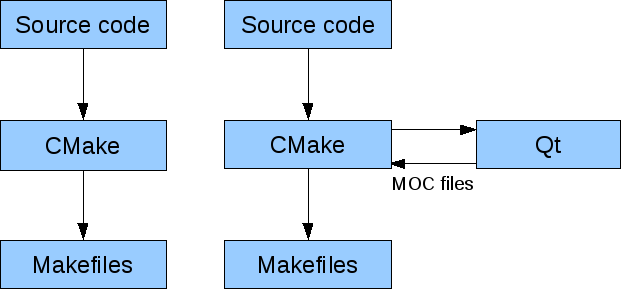
\includegraphics[width=0.5\textwidth]{images/cmake}
 \end{center}
\caption{CMake process before (left) and after (right) my modifications}
\end{figure}
